\documentclass[11pt]{aghdpl}
\usepackage[polish]{babel}
\usepackage[utf8]{inputenc}
\usepackage{enumitem}
\usepackage{listings}
\usepackage{graphicx}
\usepackage{subcaption}
\usepackage{capt-of}
\usepackage{multirow}
\usepackage{xcolor,colortbl}
\usepackage{longtable}
\usepackage{pdflscape}
\usepackage{array}
\usepackage{url}
\usepackage{varwidth}
\usepackage{hyperref}

\hypersetup{
    colorlinks,
    citecolor=black,
    filecolor=black,
    linkcolor=black,
    urlcolor=black
}

\definecolor{Gray}{gray}{0.75}
\definecolor{LightGray}{gray}{0.90}
\setitemize{itemsep=3pt,topsep=3pt,parsep=3pt,partopsep=3pt}
% Command	What it does
% \parskip
% Space between paragraphs outside of a list, and part of the space between a non-list paragraph and a list item.
% \topsep
% Extra space added to \parskip before the first and after the last item.
% \parsep
% Paragraph separation within a single item.
% \itemsep
% Extra inter-item spacing added to \parsep.
% \partopsep
% This is added to the top and/or bottom of the list if and only if there's a blank line above or below the first or last item. Leave this alone unless blank lines become a problem.
% nic nie chce dzialać
\let\oldenumerate\enumerate
\renewcommand{\enumerate}{
  \oldenumerate
  \setlength{\itemsep}{0pt}
  \setlength{\topsep}{0pt}
  \setlength{\parsep}{0pt}
  \setlength{\partopsep}{0pt}
}
\setlist[enumerate]{leftmargin=14mm}
\def \longauthor{Krzysztof Spytkowski, Magdalena Warzecha}
\author{Wojciech Kasperek, Agnieszka Maksylewicz,}
\shortauthor{W. K., A. M., K. S., M. W.}

\titlePL{Implementacja mechanizmu server-push z wykorzystaniem techniki piggy-back w technologii EJB3}
\titleEN{}

\shorttitlePL{Implementacja mechanizmu server-push z wykorzystaniem techniki piggy-back (EJB3)}
\shorttitleEN{}

\thesistype{}

\supervisor{dr Rafał Mrówka}

\degreeprogramme{Informatyka}

\subject{Wprowadzenie do wzorców projektowych}

\date{2014/2015}

\department{Katedra Informatyki Stosowanej}

\faculty{Wydział Elektrotechniki, Automatyki,\protect\\[-1mm] Informatyki i Inżynierii Biomedycznej}
\makeatletter
\newcommand*{\compress}{\@minipagetrue}
\makeatother
\newcommand{\tableEnumerateBegin}{  \noindent\par
\vspace{-\baselineskip}
\compress\begin{enumerate}}
\newcommand{\tableEnumerateEnd}{\end{enumerate}\vspace{-\baselineskip}\vspace{-\baselineskip}}
%---------------------------------------------------------------------------

\begin{document}

\titlepages
\vspace*{-20mm}
\tableofcontents
\clearpage

\chapter{Opis projektu}
Celem projektu jest implementacja mechanizmu server-push przy użyciu techniki piggy-back, wykorzystując odpowiednie wzorce projektowe. Językiem implementacji jest Java EE (EJB3). Na~wstępie warto zapoznać się z~podstawowymi pojęciami dotyczącymi tematu.


\section{Server-push}
Server-push to~mechanizm umożliwiający serwerowi wysyłać dane do~klienta. Należy jednak pamiętać, że~połączenie nawiązywane jest zawsze przez klienta, przez co~nie jest możliwe proste wysyłanie oczekiwanych danych przez serwer bez interakcji z~klientem.

Istnieje klika metod pozwalających osiągnąć zamierzony efekt. Są~to:
\begin{description}
 \item[pooling] odpytywanie serwera w~stałym krótkim interwale czasowym
 \item[piggy-back] opisany w~kolejnej sekcji
 \item[comet] podtrzymywanie zapytania przez serwer do~momentu wygaśnięcia czasowego (timeout) lub do~pojawienia się oczekiwanych informacji (zwracanych klientowi)
\end{description}


\section{Piggy-back}
Nazwa techniki może zostać przetłumaczona jako~``jazda na~barana''. Może to~sugerować sposób działania metody. 

Klient wysyła zapytanie do~serwera w~celu wykonania pewnej operacji. Serwer ma~za~zadanie wysłać odpowiedź zgodną z~oczekiwaniami klienta. Dodatkowo jednak, jeśli posiada inne informacje do~przekazania klientowi, dołącza je~do odpowiedzi, tworząc \textit{mixed response}.
\begin{center}
 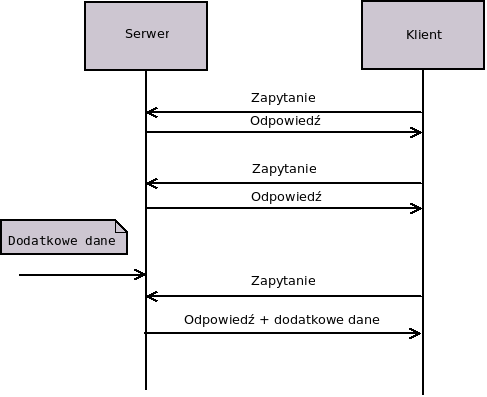
\includegraphics[width=8cm]{piggy}
\end{center}

Jest to~rozwiązanie znacznie wydajniejsze niż~\textit{pooling}, ze~względu na~brak użycia dodatkowych zasobów klienta. Ma~jednak swoje wady, ponieważ informacje mogą nigdy nie dotrzeć do~klienta (w~przypadku nie wykonania zapytania) lub też~dotrzeć po~długim czasie. Lepszym rozwiązaniem jest \textit{comet}.

\section{Opis pomysłu}
Ze względu na~dość ogólny charakter tematu, stworzyliśmy koncepcję pozwalającą pokazać działanie mechanizmu piggy-back oraz wykorzystanie wzorców projektowych.

Opisywana aplikacja to~program do~obsługi barów - z~punktu widzenia barmana. Konkretnie, występują dwa rodzaje barów: plebejski i~luksusowy. Mają one w~swojej ofercie kilka typów napojów wyskokowych: piwa (jasne, ciemne) oraz~drinki (Bloody Mary, Pina Colada). W~zależności od~typu baru, barman korzysta z~różnych przepisów przygotowywania napojów (w~szczególności w~barze plebejskim zamiast części alkoholu dolewa wodę). 

Bary przechowują stan - aktualnie posiadaną ilość produktów potrzebnych do~tworzenia napojów. Może się~zdarzyć, że~zabraknie jakiegoś składnika koniecznego do~przygotowania zamówienia. W~takim wypadku bar wysyła zamówienie do~dostawcy produktów, który natychmiastowo dostarcza brakujący składnik (jeśli jest to~możliwe). 

W~celu zaprezentowania samego mechanizmu piggy-back została dodana możliwość obserwowania zamówień. Barman może wybrać bary, z~których chce otrzymywać informacje o~składanych zamówieniach. Dane te~są~dostarczane do~przeglądarki w~przypadku wykonania innego zapytania.

Warto dodać, że~barman to~pojedyncza sesja klienta.
\chapter{Architektura}
\section{Zarys}
Aplikacja została stworzona przy użyciu klasycznej dla Javy EE architektury.

\begin{center}
 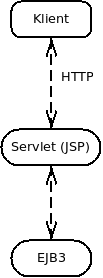
\includegraphics[width=6cm]{arch}
\end{center}

Jest to~model trójwarstwowy, składający się~z~widoku (strona klienta, interfejs graficzny), prezentera (servlety, JSP) i~modelu, czyli logiki i~danych reprezentowanych przez EJB. W~przypadku naszej aplikacji używane są~jedyne \textit{session beans}, które utożsamiane są~z~logiką aplikacji. Projekt nie wymagał użycia bazy danych.

Każde zapytanie klienta jest przechwytywane przez servlet, który przekazuje je~do~logiki aplikacji. Wynik działania logiki jest przetwarzany na~odpowiedź i~odsyłany do~klienta. Używana jest głównie komunikacja asnychroniczna (AJAX - Asynchronous JavaScript and XML).

\section{Użyte narzędzia}
Do~implementacji posłużyliśmy się:
\begin{itemize}
 \item Netbeans IDE 7.4,
 \item serwer aplikacyjny GlassFish Server 4.0,
 \item Jave EE 7.0,
 \item Bootstrap,
 \item JavaScript + JQuery.
\end{itemize}



\chapter{Wzorce projektowe}
W ramach projektu zaimplementowane zostało kilka wzorców projektowych.
\section{Chain of responsibility}
Implementacja wzorca ma~symulować rzeczywistych dostawców produktów. Bar, w~przypadku braku jakiegoś produktu, używa \textit{nadzorcy dostawców} (ProviderMain) w~celu wysłania żądania dostarczenia produktu. ProviderMain przekazuje zapytanie pierwszemu dostawcy;
kolejni dostawcy przekazują je~dalej, jeśli nie potrafią go~zrealizować.

\subsection{Szczegóły implementacji}
Dostawcy są~implementowani przy pomocy \textit{stateless bean}, ponieważ reprezentują część logiki i~nie przechowują stanu. Nadzorca zawiera wstrzyknięte wszystkie elementy łańcuch, z~których tworzy ciąg zależności. Również jest to~\textit{stateless bean}.

Razem z~treścią zapytania przekazywany jest obiekt pytający, który musi implementować interfejs ProductReceiver. Przy realizacji zlecenia jest on~bezpośrednio wykorzystywany.
\begin{center}
 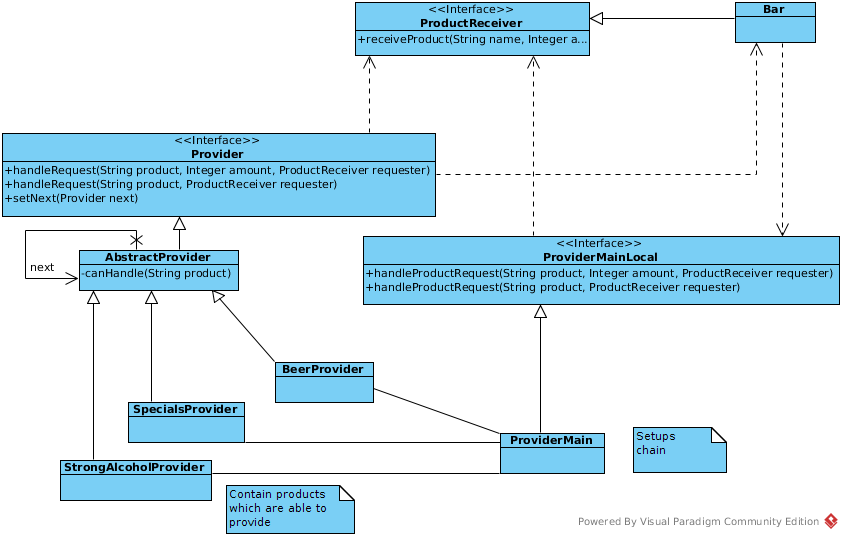
\includegraphics[width=16cm]{chain}
\end{center}

Zastosowanie wzorca jest uzasadnione, ponieważ z~punktu widzenia baru nie jest ważne, który dostawca obsłuży zamówienie. Ponadto, nie ma~konieczności znania wszystkich dostawców.

\section{PublishSubscribe}
Implementacja wzorca ma~zapewnić Barmanom (subscribers) możliwość obserwowania zamówień w~różnych Barach (publishers). Bar, obsługując zamówienie, tworzy zdarzenie, które wysyła do~PublishService. PublishService korzysta z~informacji o~subskrybentach udostępnianych przez FilterUnit, i~przesyła do nich dane. Subskrybenci mogą rejestrować się~do~danego tematu poprzez SubscribeService, który uaktualnia dane przechowywane w~FilterUnit.

\subsection{Szczegóły implementacji}
FilterUnit jest implementowany jako \textit{singleton bean}, ponieważ musi przechowywać stan i~jest pojedynczym obiektem. Z~kolei PublishService i~SubscribeService to~\textit{stateless bean} reprezentujące część logiki. Interfejsy Publisher i~Subscriber umożliwiają korzystanie z~serwera PubSub wielu różnym klasom. Przekazywane wiadomości muszą implementować interfejs Event.

\begin{center}
 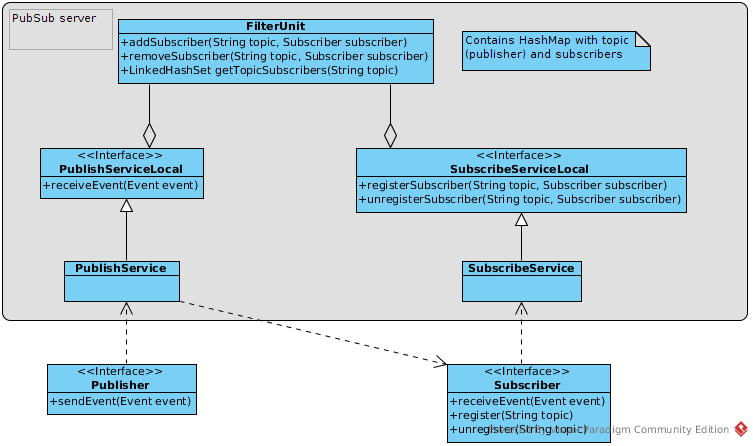
\includegraphics[width=14cm]{pubsub}
\end{center}

Wzorzec pozwala uniezależnić nadawców od~odbiorców, ponieważ wysyłane wiadomości są~opatrywane nazwą nadawcy (tematem), a~nie danymi odbiorców. Ponadto odpowiedzialność za~dostarczenie informacji jest oddelegowana poza klasę tworzącą wiadomość. 

Jedyną możliwością komunikacji między nadawcami a~odbiorcami są~wiadomości.

\chapter{Przykład}
\begin{center}
 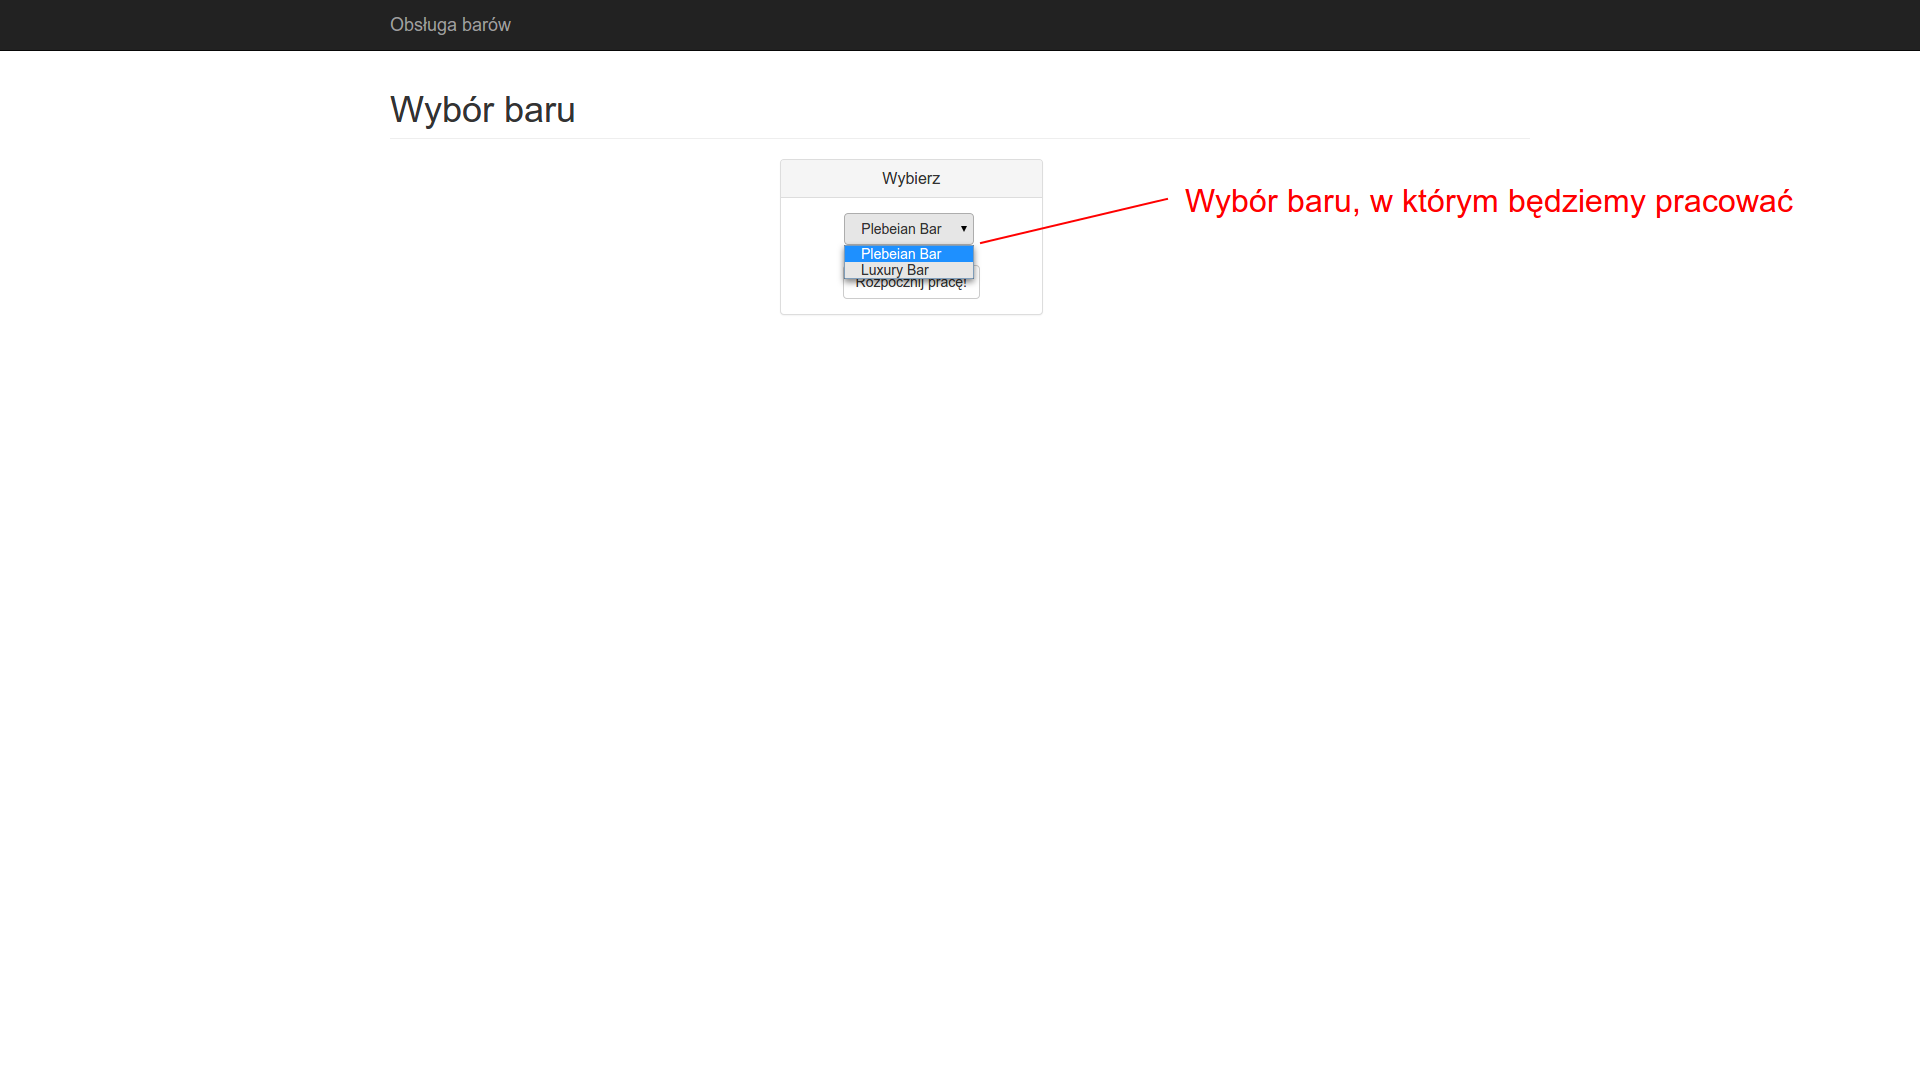
\includegraphics[width=16cm]{zrzut1}
\end{center}
\begin{center}
 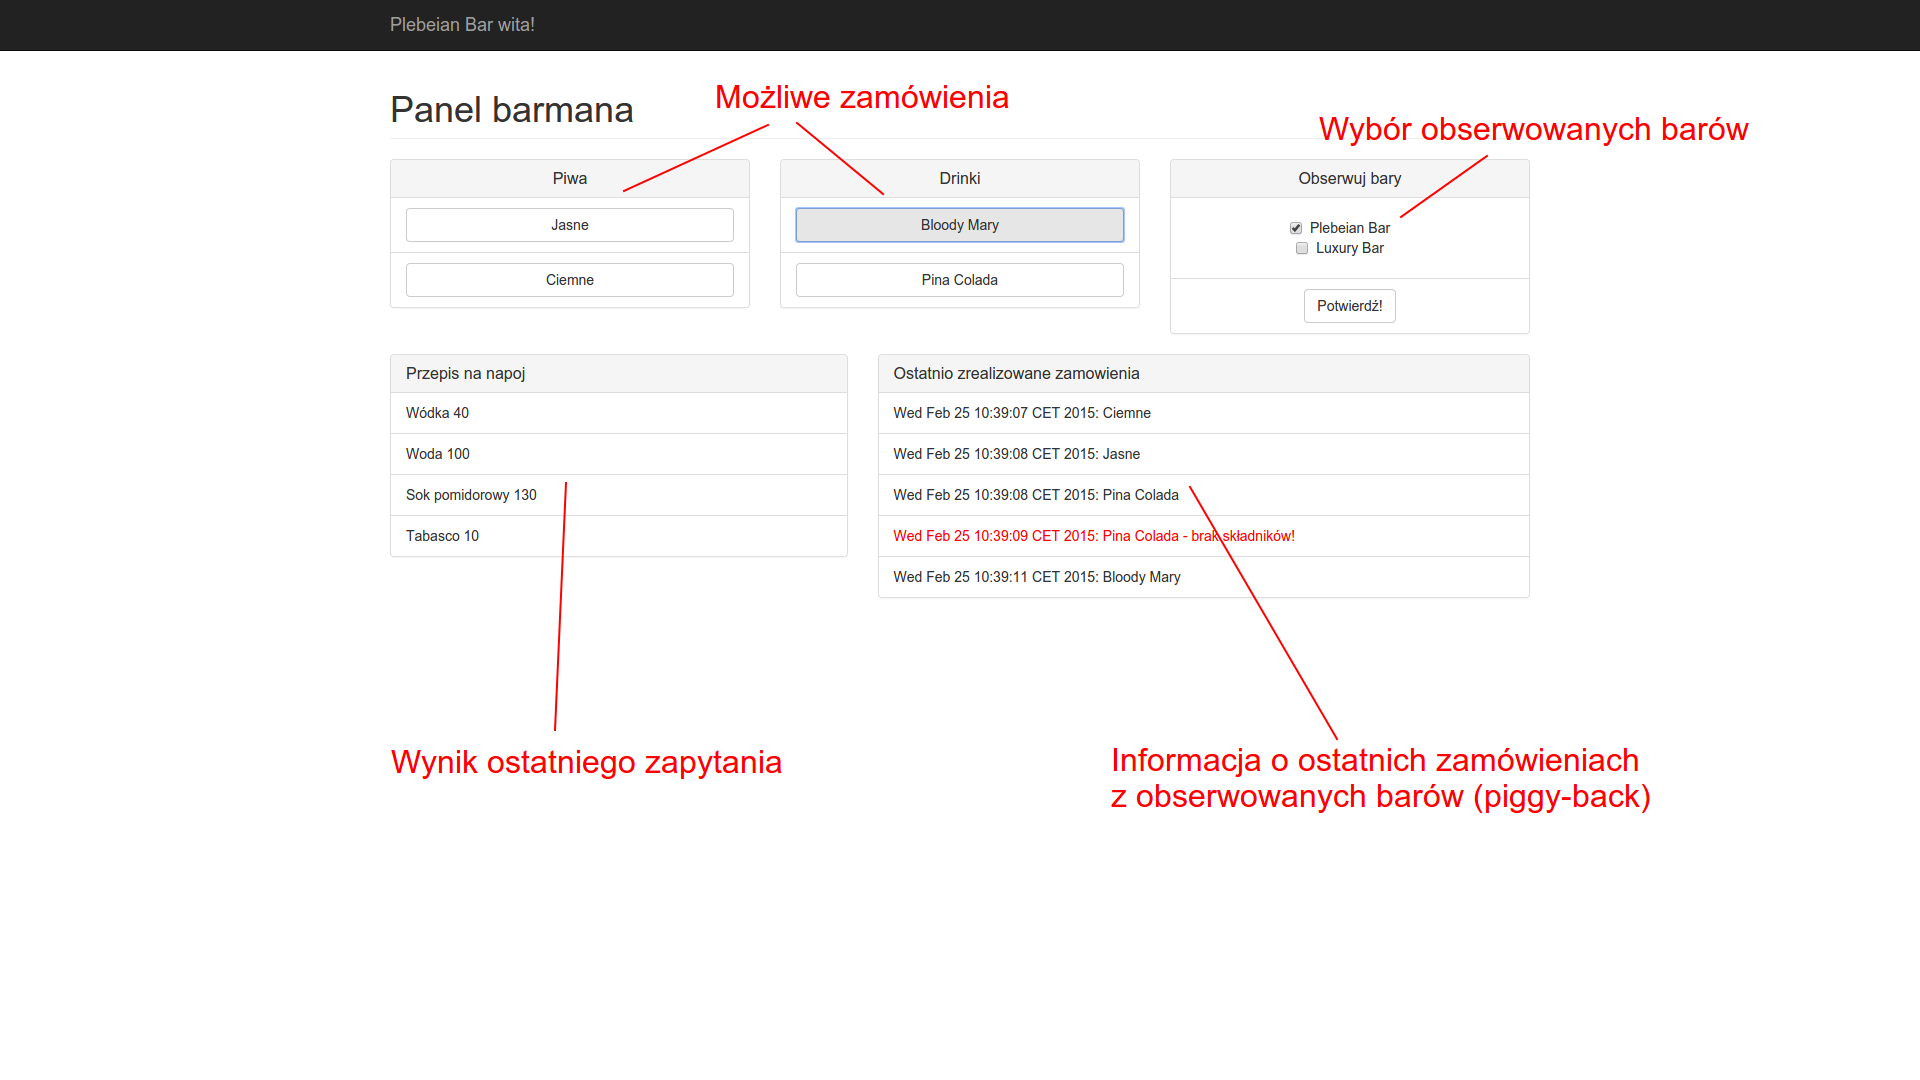
\includegraphics[width=16cm]{zrzut2}
\end{center}

\end{document}